% -*- TeX-master: "report" -*-

\section{Experiments}

This section presents quantitative data about the ideas presented in previous sections.  This data was collected using the Siemens test suite \cite{257766} as maintained by the Galileo Software-artifact Infrastructure Repository (SIR) \cite{Do05,SAI}.  There are two configurable parameters for the experiments: the sampling rate and the $\effort$ cutoff (described in \autoref{sec-metrics}).  Unless specified, the default sampling rate is 1 (i.e., complete data collection) and the default $\effort$ is 5\% (only predicates that are reachable from each other by exploring less than 5\% of the program are considered).  Each Siemens application is available in multiple variants with different bugs: as few as 9 variants of \prog{schedule2} and as many as 41 variants of \prog{tcas}.  We report aggregate results by averaging the relevant measures across all variants of each Siemens application.

\subsection{Top Scoring Predicates}

\label{sec-quant}
\begin{figure}
  \centering
  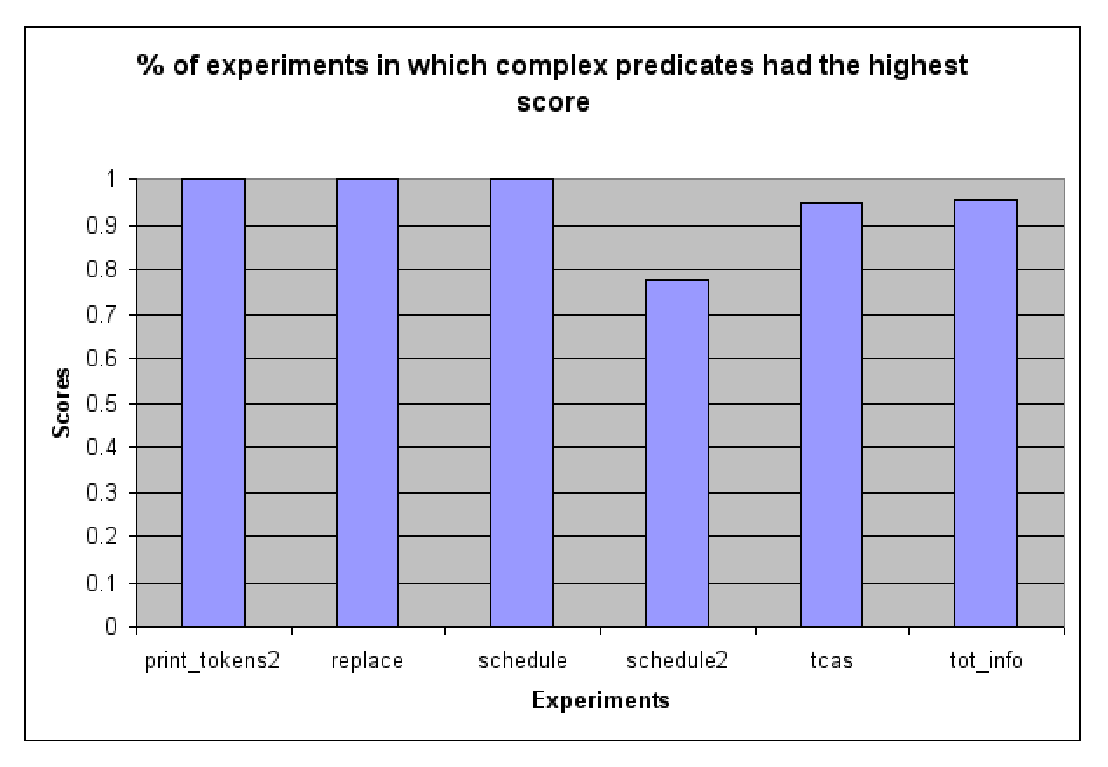
\includegraphics{charts/top-pred}
  \caption{Fraction of buggy application variants having a complex predicate as the top-scoring predictor}
  \label{fig-top-pred}
\end{figure}

\autoref{fig-top-pred} plots the percentage of variants within each program for which a complex predicate had the highest score among all predicates.  The value is 100\% for \prog{print\_tokens2}, \prog{replace} and \prog{schedule} and is close to 100\% for the other programs.  The results shown in \autoref{fig-top-pred} combined with the case studies in \autoref{sec-qual} demonstrates the usefulness of complex predicates.

\subsection{Effectiveness of Pruning}
\label{sec-effectprune}
\begin{figure}
  \centering
  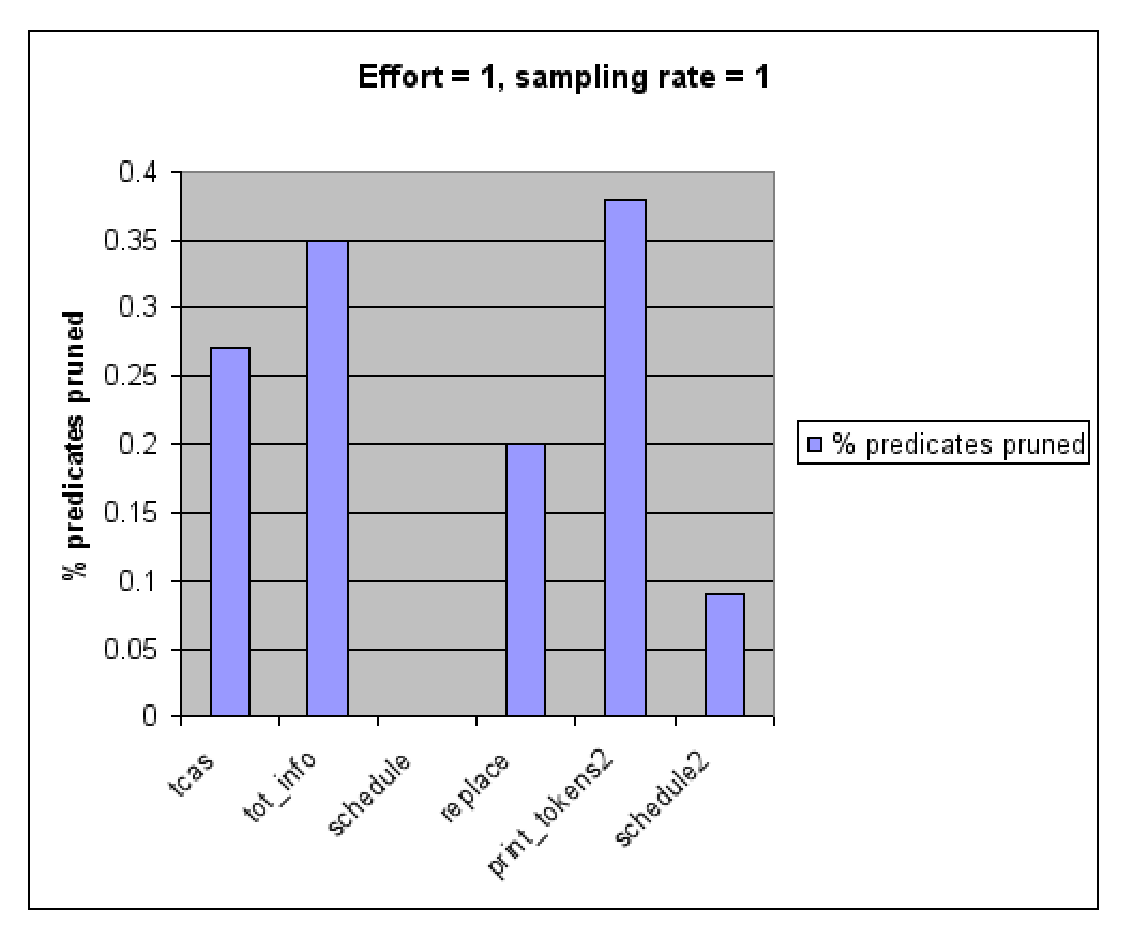
\includegraphics{charts/pruning}
  \caption{Avoiding computing exact scores by pruning complex predicates.  ``Overall'' summarizes the entire Siemens suite.}
  \label{fig-pruning}
\end{figure}

Even when restricted to binary conjunction and disjunction, complex predicates could substantially increase the analysis workload if na\"ively implemented.  \autoref{sec-metrics} suggests heuristics for pruning complex predicates which are unlikely to be useful or understandable to a programmer, while \autoref{sec-pruning} describes how to compute an upper bound on a predicate's score.  \autoref{fig-pruning} shows that these measures are highly effective in practice.  On average, 57\% of candidate complex predicates are discarded because the $\effort$ as defined in \autoref{def-effort} would require traversing more than 5\% of the application code.  A further 14\% of complex predicates are pruned because the upper bounds of their $\Importance$ scores, computed per \autoref{sec-pruning}, are lower than the scores of their constituent simple predicates.  Only 29\% of complex predicates remain to have their exact scores computed, of which roughly a sixth (5\% of the initial pool) are retained as potentially interesting bug predictors.  Thus we find that the techniques proposed earlier significantly reduce the computational load required to identify a useful, high-scoring subset of complex predicates.

\subsection{Effect of Effort}

\begin{figure}
  \centering
  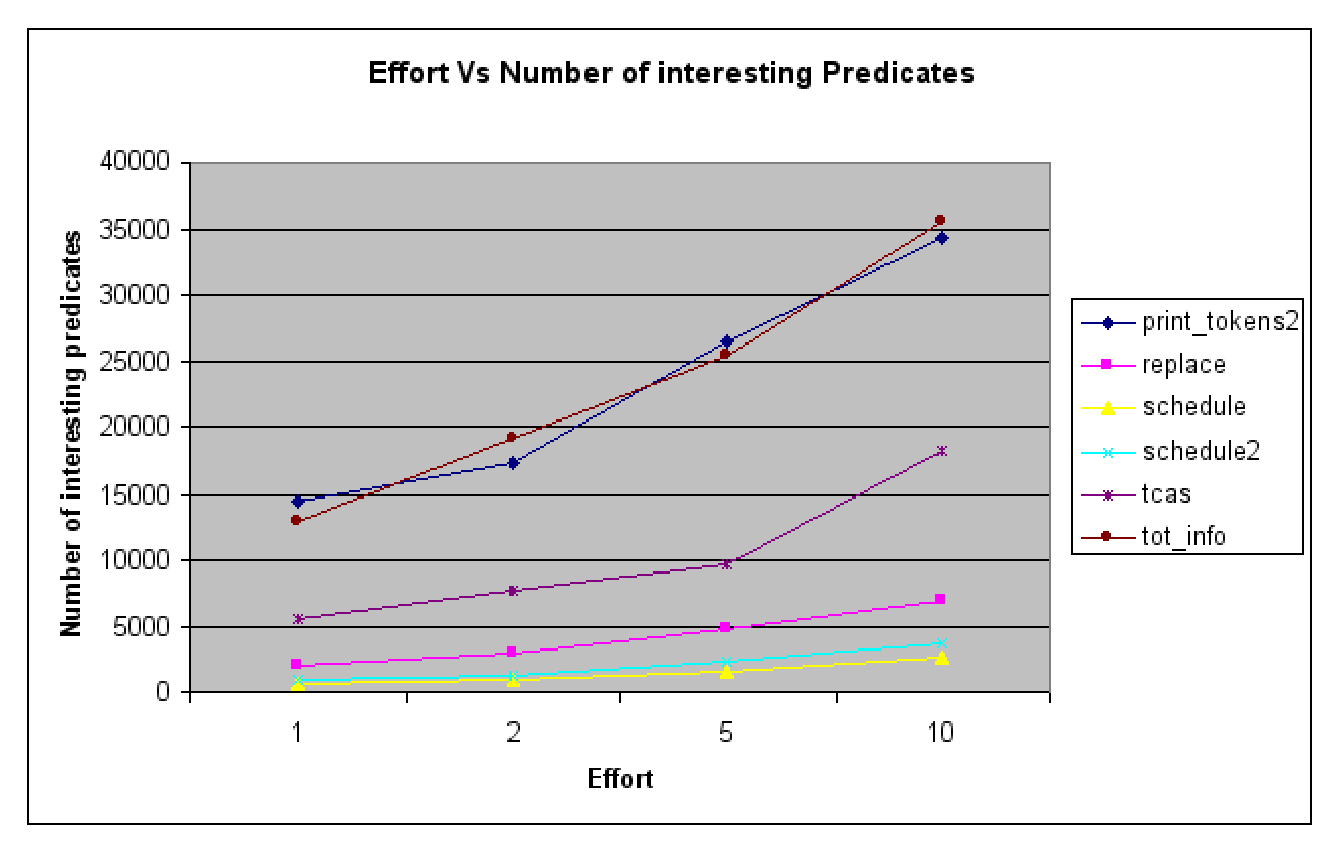
\includegraphics{charts/effort}
  \caption{Variation of number of interesting predicates with $\effort$}
  \label{fig-effort}
\end{figure}

\autoref{fig-effort} has one curve for each program showing how the number of interesting predicates (\autoref{dfn3}) varies at four different values - 1, 2, 5, 10 for $\effort$.  As expected, as $\effort$ increases more predicates are evaluated and so more interesting predicates are found.

\subsection{Effect of Sampling Rate}
\label{sec-sampling}

\begin{figure*}
  \centering
  \newcommand{\plot}[2]{\subfloat[\prog{#1}]{\includegraphics{charts/sampling-#2}}}
  \section{Sparse Random Sampling and Complex Predicates}
\label{sec-sampling}
  \caption{Sampling rate vs. number of interesting predicates}
  \label{fig-sampling}
\end{figure*}

The dependence between sampling rate and the number of interesting predicates (both complex and simple) is plotted in \autoref{fig-sampling}.  \autoref{fig-sampling} has one chart per program with sampling rates in the $x-$axis and the average number of interesting conjunctions, disjunctions and simple predicates in the $y-$axis.  The number of interesting disjunctions is always very low (order of tens) compared to interesting conjunctions.  So the plot for interesting complex predicates closely follows the plot for conjunctions.  At sampling rates lower than \nicefrac{1}{10}, there is a sharp drop in the number of interesting conjunctions.  This is because the chance of observing both components of a conjunction within a single run falls with the square of the sampling rate.  Despite the sharp drop, the number of interesting conjunctions is still comparable to the number of interesting simple predicates even at \nicefrac{1}{1000} sampling.  This shows interesting complex predicates can still be found at sparse but realistic sampling rates.

A puzzling trend in \autoref{fig-sampling} is that the curves raise for a 
brief interval before dropping off.  This trend occurs for conjunctions and 
disjunctions as well as for simple predicates.  Also it is consistent across
all applications.  The bumps in the conjunction and disjunction curves could
be attributed to the bump in the simple predicates curve.  An increase
in the number of interesting simple predicates is likely to produce a steeper 
increase in the number of interesting complex predicates, especially because
the additional simple predicates are likely to be redundant (as explained
later).

This surprising trend in the simple predicates was previously undiscovered
and seemed counterintuitive in the beginning.  But drilling down into our
experimental results revealed two scenarios where this could happen.

\begin{enumerate}
\item The first scenario happens due to an adhoc, but perfectly reasonable
elimination of seemingly identical predicates.  As an example, consider the
predicates $p$: \texttt{a == b} and $q$: \texttt{a >= b}.  If they have the
same score, it is useful to just retain $p$ as it is a more stringent
condition than $q$ but still has the same score.  However it does not mean
that \texttt{a > b} was never true.  \texttt{a > b} may be observed  during 
some runs but does not affect the outcome of \texttt{a >= b} if \texttt{a == b}
also happens to be true in that run.  However, at sampling rates lower than
1, only \texttt{a > b} may be observed in some runs and hence the number of
runs in which $p$ and $q$ are observed \emph{true}, and consequently their
scores may be different.  Thus, the adhoc elimination heuristic performs 
less effectively at lower sampling rates, leading to an increase in the 
number of interesting simple predicates

\item To understand the second scenario, consider a predicate $p$ for which
\begin{eqnarray*}
 \obs{S}{p} &=& S(p) \\
 \obs{F}{p} &=& F(p) \\
\end{eqnarray*}
In other words, $p$ was true atleast once in every run in which it was 
observed atleast once.  From \autoref{eqn1}, $\Increase(p) = 0$.  In a run 
in which $p$ was observed, it may also be \emph{false} atleast once.  As we
reduce the sampling rates, only the \emph{false} occurences may be recorded
in some runs and hence the two equalities may no longer hold.  As a result
$\Increase(p)$ may be nonzero and if it becomes positive a predicate that
was not interesting at higher sampling rates becomes interesting at lower 
sampling rates.
\end{enumerate}

The first scenario was found to be more prevalent than the second during
exploration of the results of an experiment (\prog{tot\_info} version 1).

